\documentclass{ximera}
%% You can put user macros here
%% However, you cannot make new environments

\listfiles

\graphicspath{{./}{firstExample/}{secondExample/}}

\usepackage{tikz}
\usepackage{tkz-euclide}
\usepackage{tikz-3dplot}
\usepackage{tikz-cd}
\usetikzlibrary{shapes.geometric}
\usetikzlibrary{arrows}
\usetkzobj{all}
\pgfplotsset{compat=1.13} % prevents compile error.

%\renewcommand{\vec}[1]{\mathbf{#1}}
\renewcommand{\vec}{\mathbf}
\newcommand{\RR}{\mathbb{R}}
\newcommand{\dfn}{\textit}
\newcommand{\dotp}{\cdot}
\newcommand{\id}{\text{id}}
\newcommand\norm[1]{\left\lVert#1\right\rVert}
 
\newtheorem{general}{Generalization}
\newtheorem{initprob}{Exploration Problem}

\tikzstyle geometryDiagrams=[ultra thick,color=blue!50!black]

%\DefineVerbatimEnvironment{octave}{Verbatim}{numbers=left,frame=lines,label=Octave,labelposition=topline}



\usepackage{mathtools}


\title{Where was Eye? (part 3)} \license{CC BY-NC-SA 4.0}

\begin{document}

\begin{abstract}
We determine the location of the camera based on a photograph it took.
\end{abstract}
\maketitle

\section*{Where was Eye? (part 3)}


We will now develop a theoretical foundation for our method of figuring out the height of the camera. 

\begin{exploration}\label{exp:hideAndSeek}
Suppose Alice, Bob, Colin, Daria, and Evan are playing hide-and-seek in the school yard.  Alice is the seeker.  The diagram below shows the location of the players.  Which of the children is visible to Alice?
     \begin{image}
         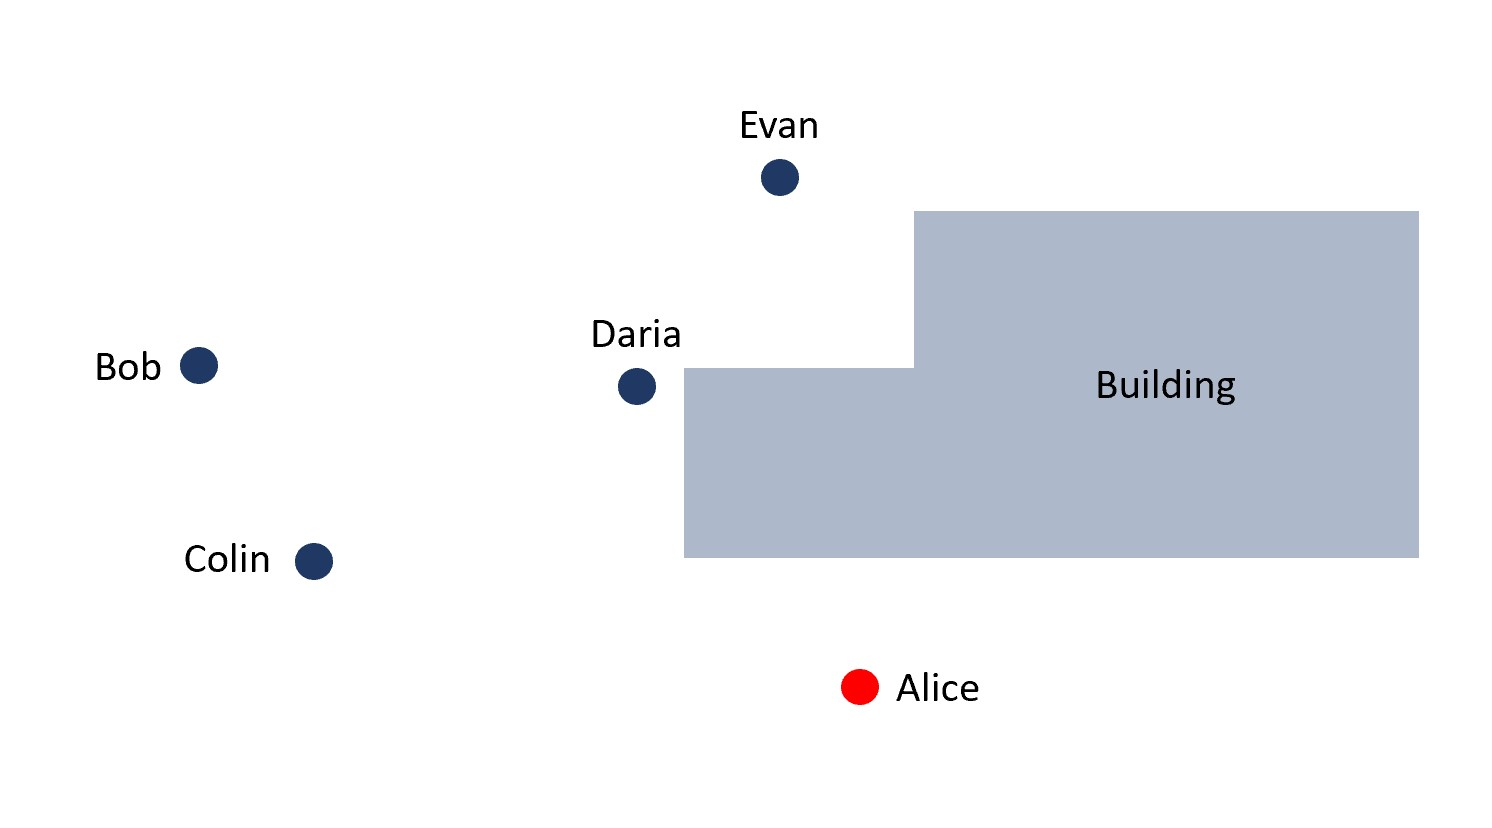
\includegraphics[width=5in]{hideAndSeek1.jpg}
\end{image}
Check the names of all the children that Alice can see.
\begin{selectAll}
\choice[correct]{Bob}
\choice[correct]{Colin}
\choice{Daria}
\choice{Evan}
\end{selectAll}

\textbf{Group Discussion Prompt:}
\emph{Articulate the reason for your choices.  If you need help formulating your thoughts, click on the arrow (below, right), and use the diagram to help you.}

\begin{expandable}
    \begin{image}
         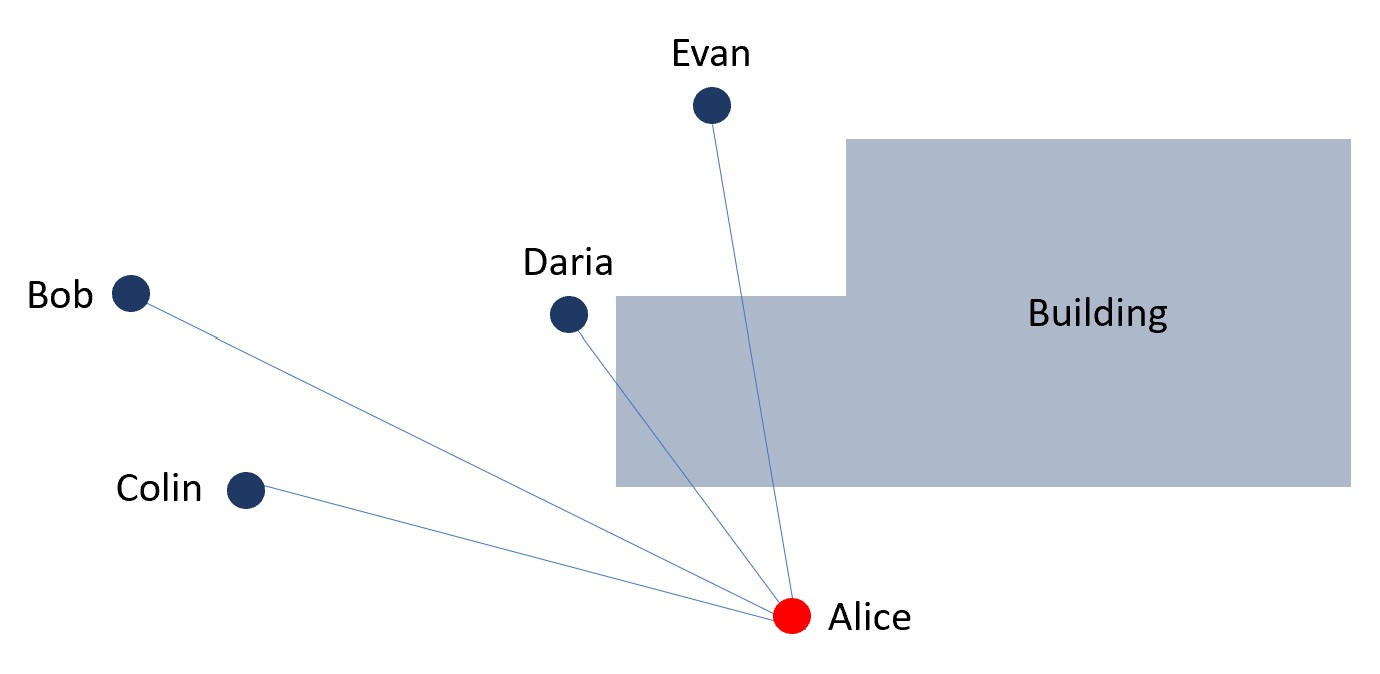
\includegraphics[width=4in]{hideAndSeek2.jpg}
\end{image}
\end{expandable}
\end{exploration}

The above exploration intuitively established a very important fact: we see along straight lines.  These lines are called \emph{lines of sight}.
\begin{image}
         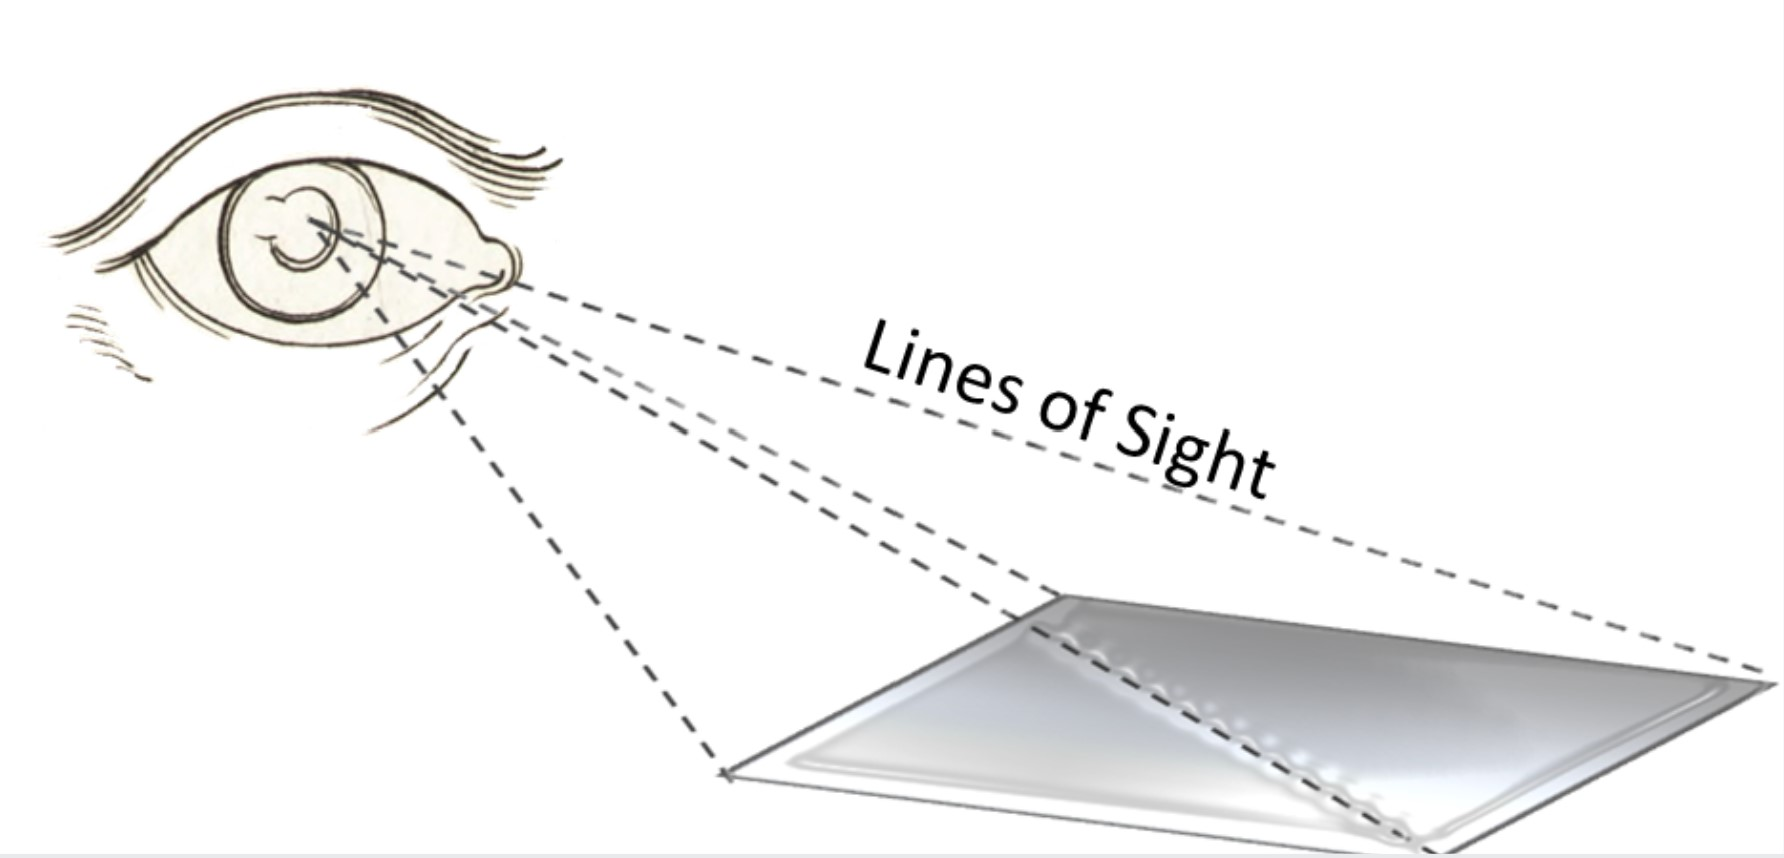
\includegraphics[width=3in]{linesOfSight.jpg}
\end{image}

\subsection*{Picture Planes}
To understand how lines of sight can help us create a realistic picture, imagine a canvas made of glass.  If you position the glass canvas in front of the object you want to draw, you can simply trace the object onto the glass with a marker.  We will call the glass canvas a \emph{picture plane}.

Take a look at the photograph below.  The student in the photo has just finished tracing the cube onto the glass.  From her point of view, the tracing matches up with the cube. 

\begin{image}
         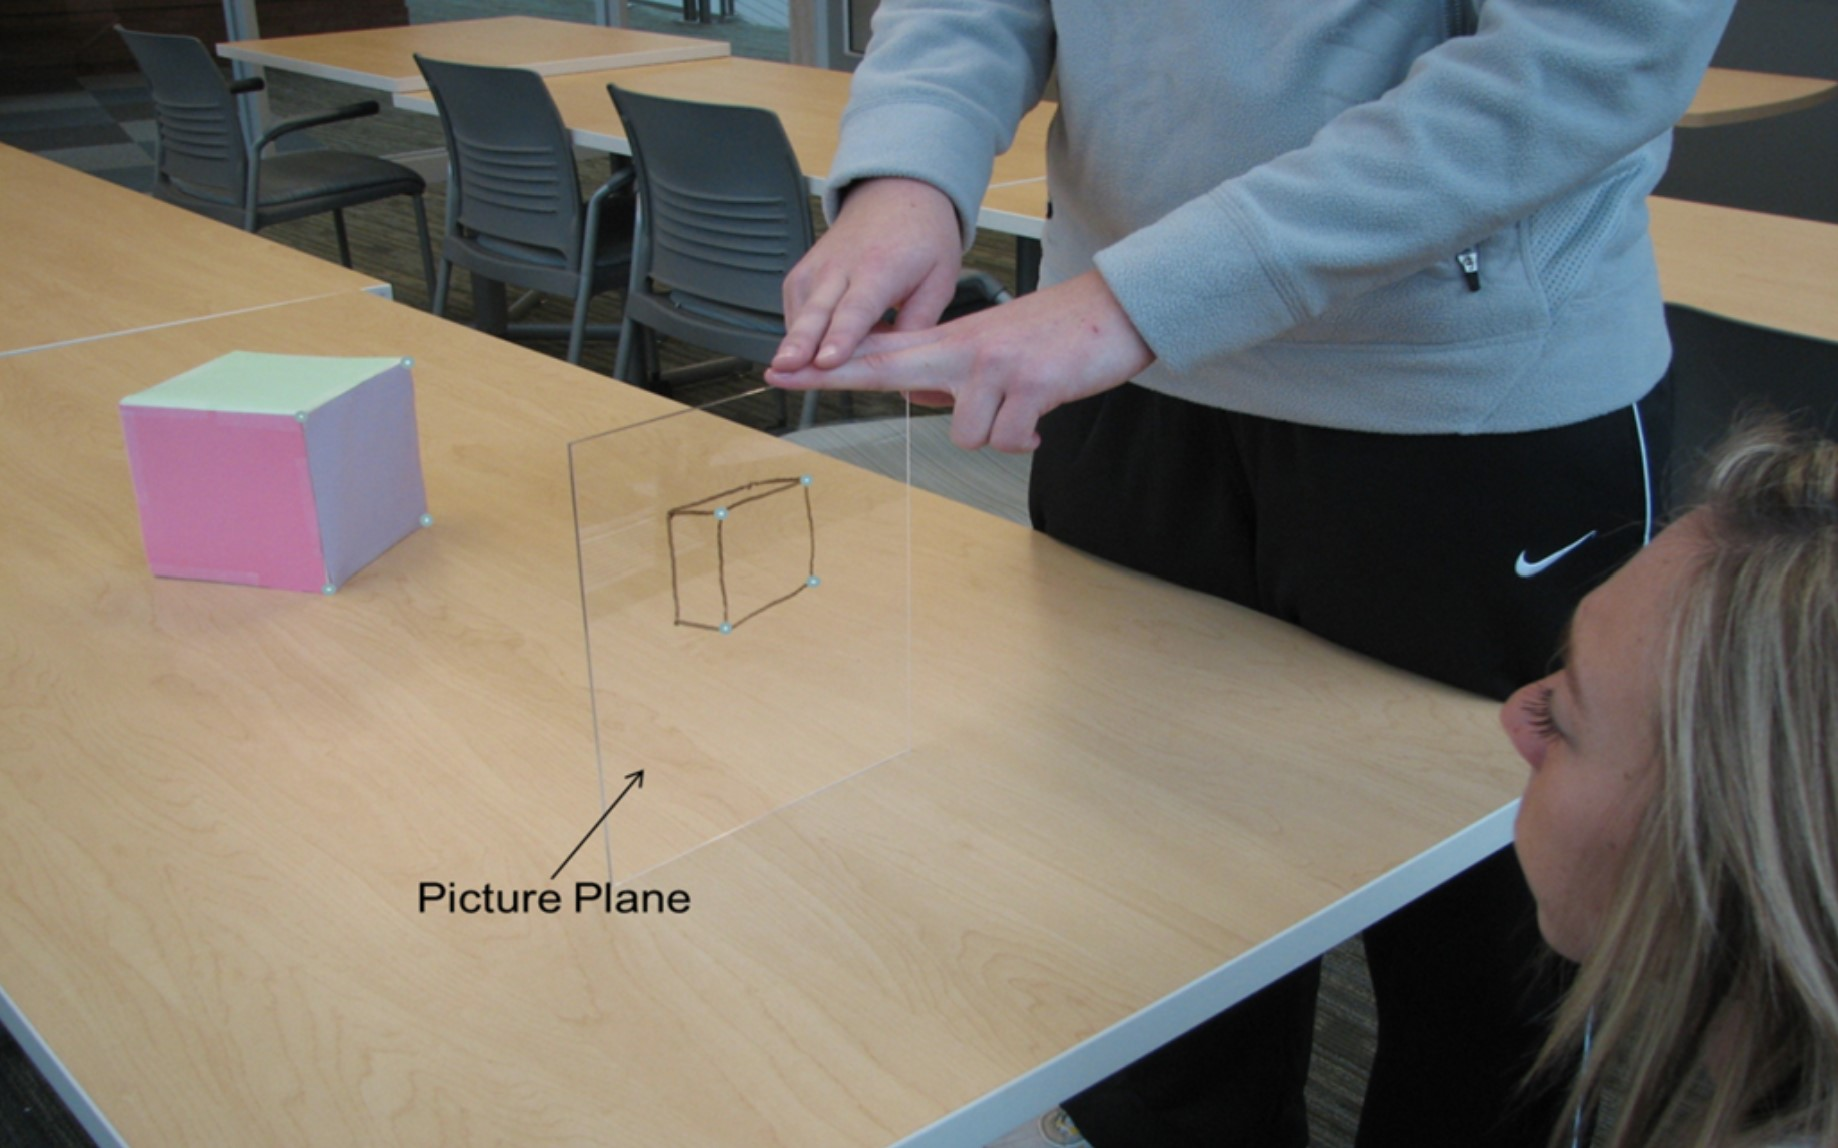
\includegraphics[width=4in]{cube.jpg}
\end{image}

Now let’s draw lines of sight that connect the corners of the cube with the eye. The line of sight from each corner of the cube passes through its image on the glass!  

\begin{image}
         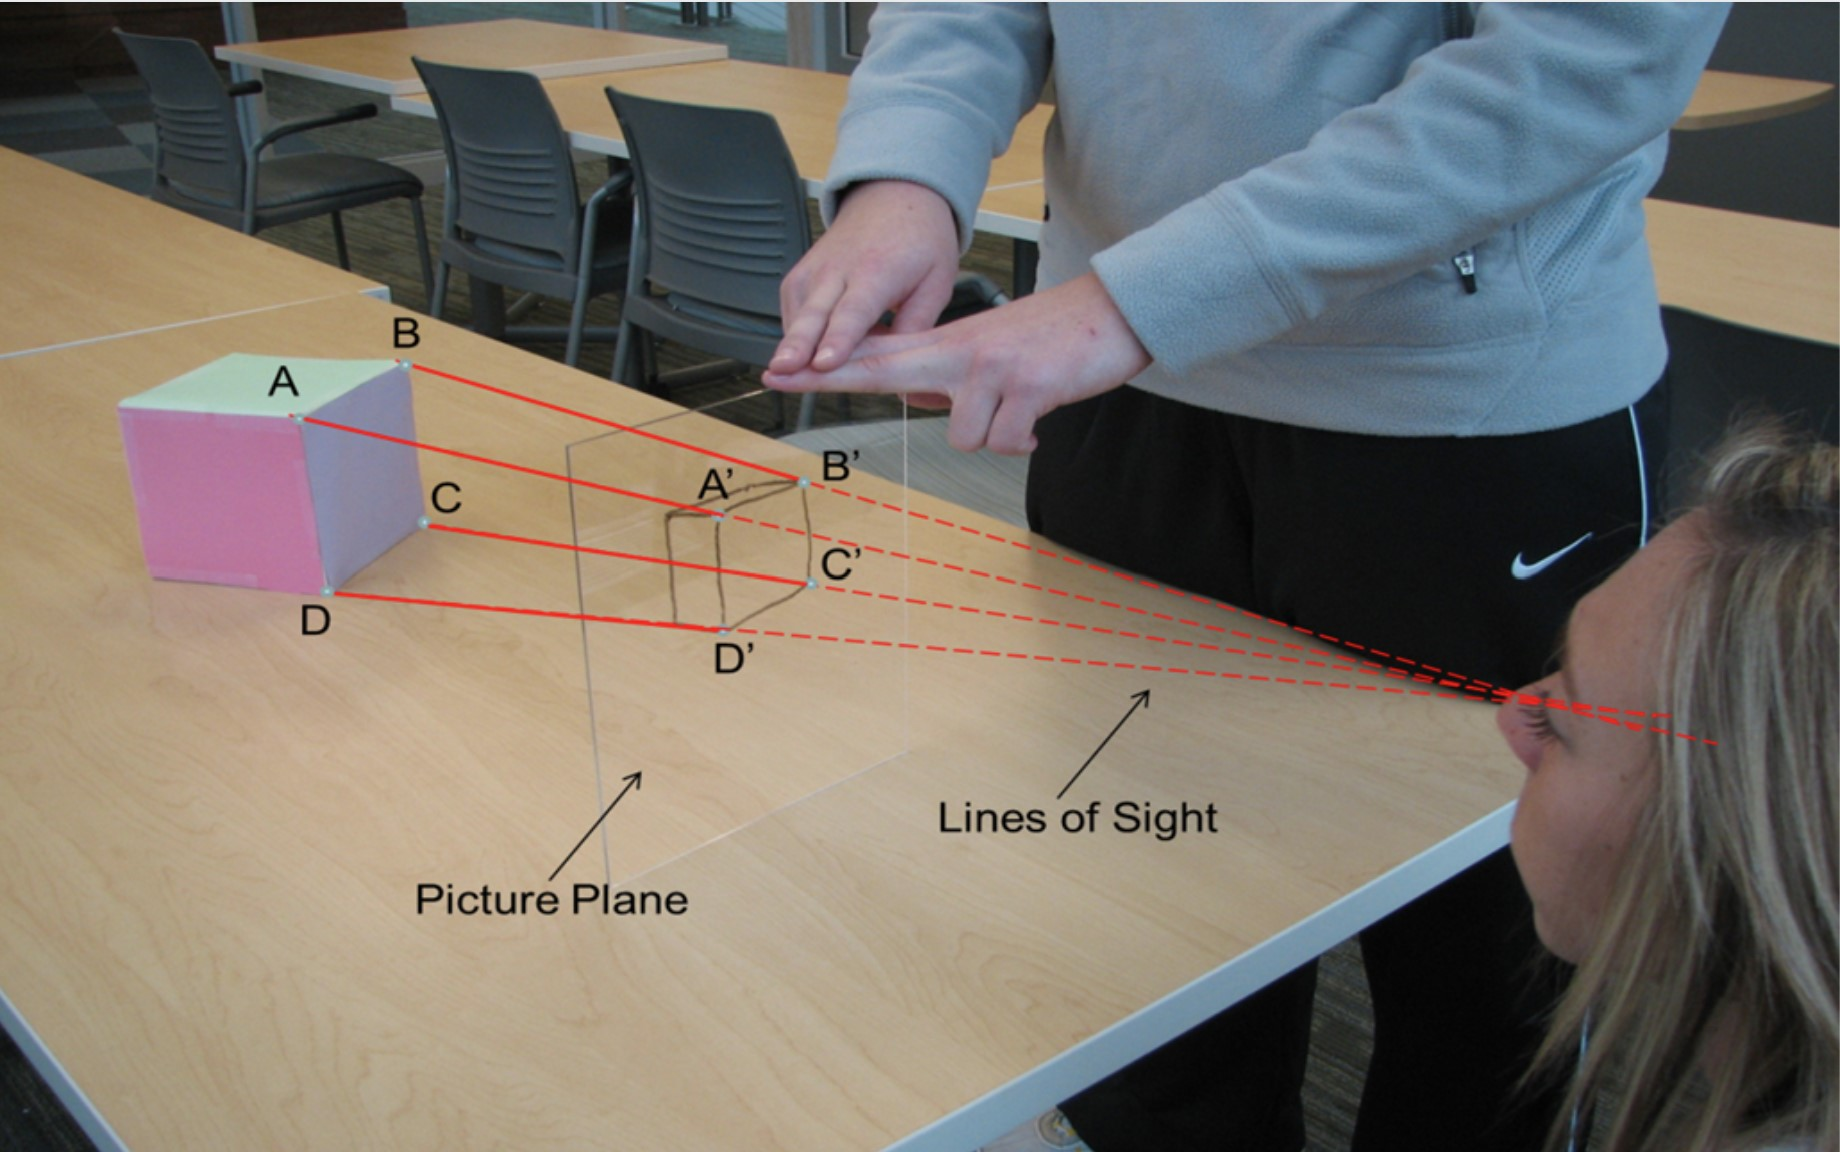
\includegraphics[width=4in]{cubeLines.jpg}
\end{image}

This principle allows artists and computer programmers to draw any object from the point of view of an imaginary eye.  If we were to place a camera where the student's eye was located, the picture taken by the camera would match the tracing on the glass.

\subsection*{Vanishing Point and the Height of the Eye (Camera)}
Now that we know about lines of sight and the picture plane, we are ready to figure out why the method we discovered and tested in the first two parts of the activity actually works.

\begin{exploration}\label{exp:punchline}
Recall that when a life-sized version of an image was used, the height of the triangle was equal to the height of the camera.

\begin{image}
         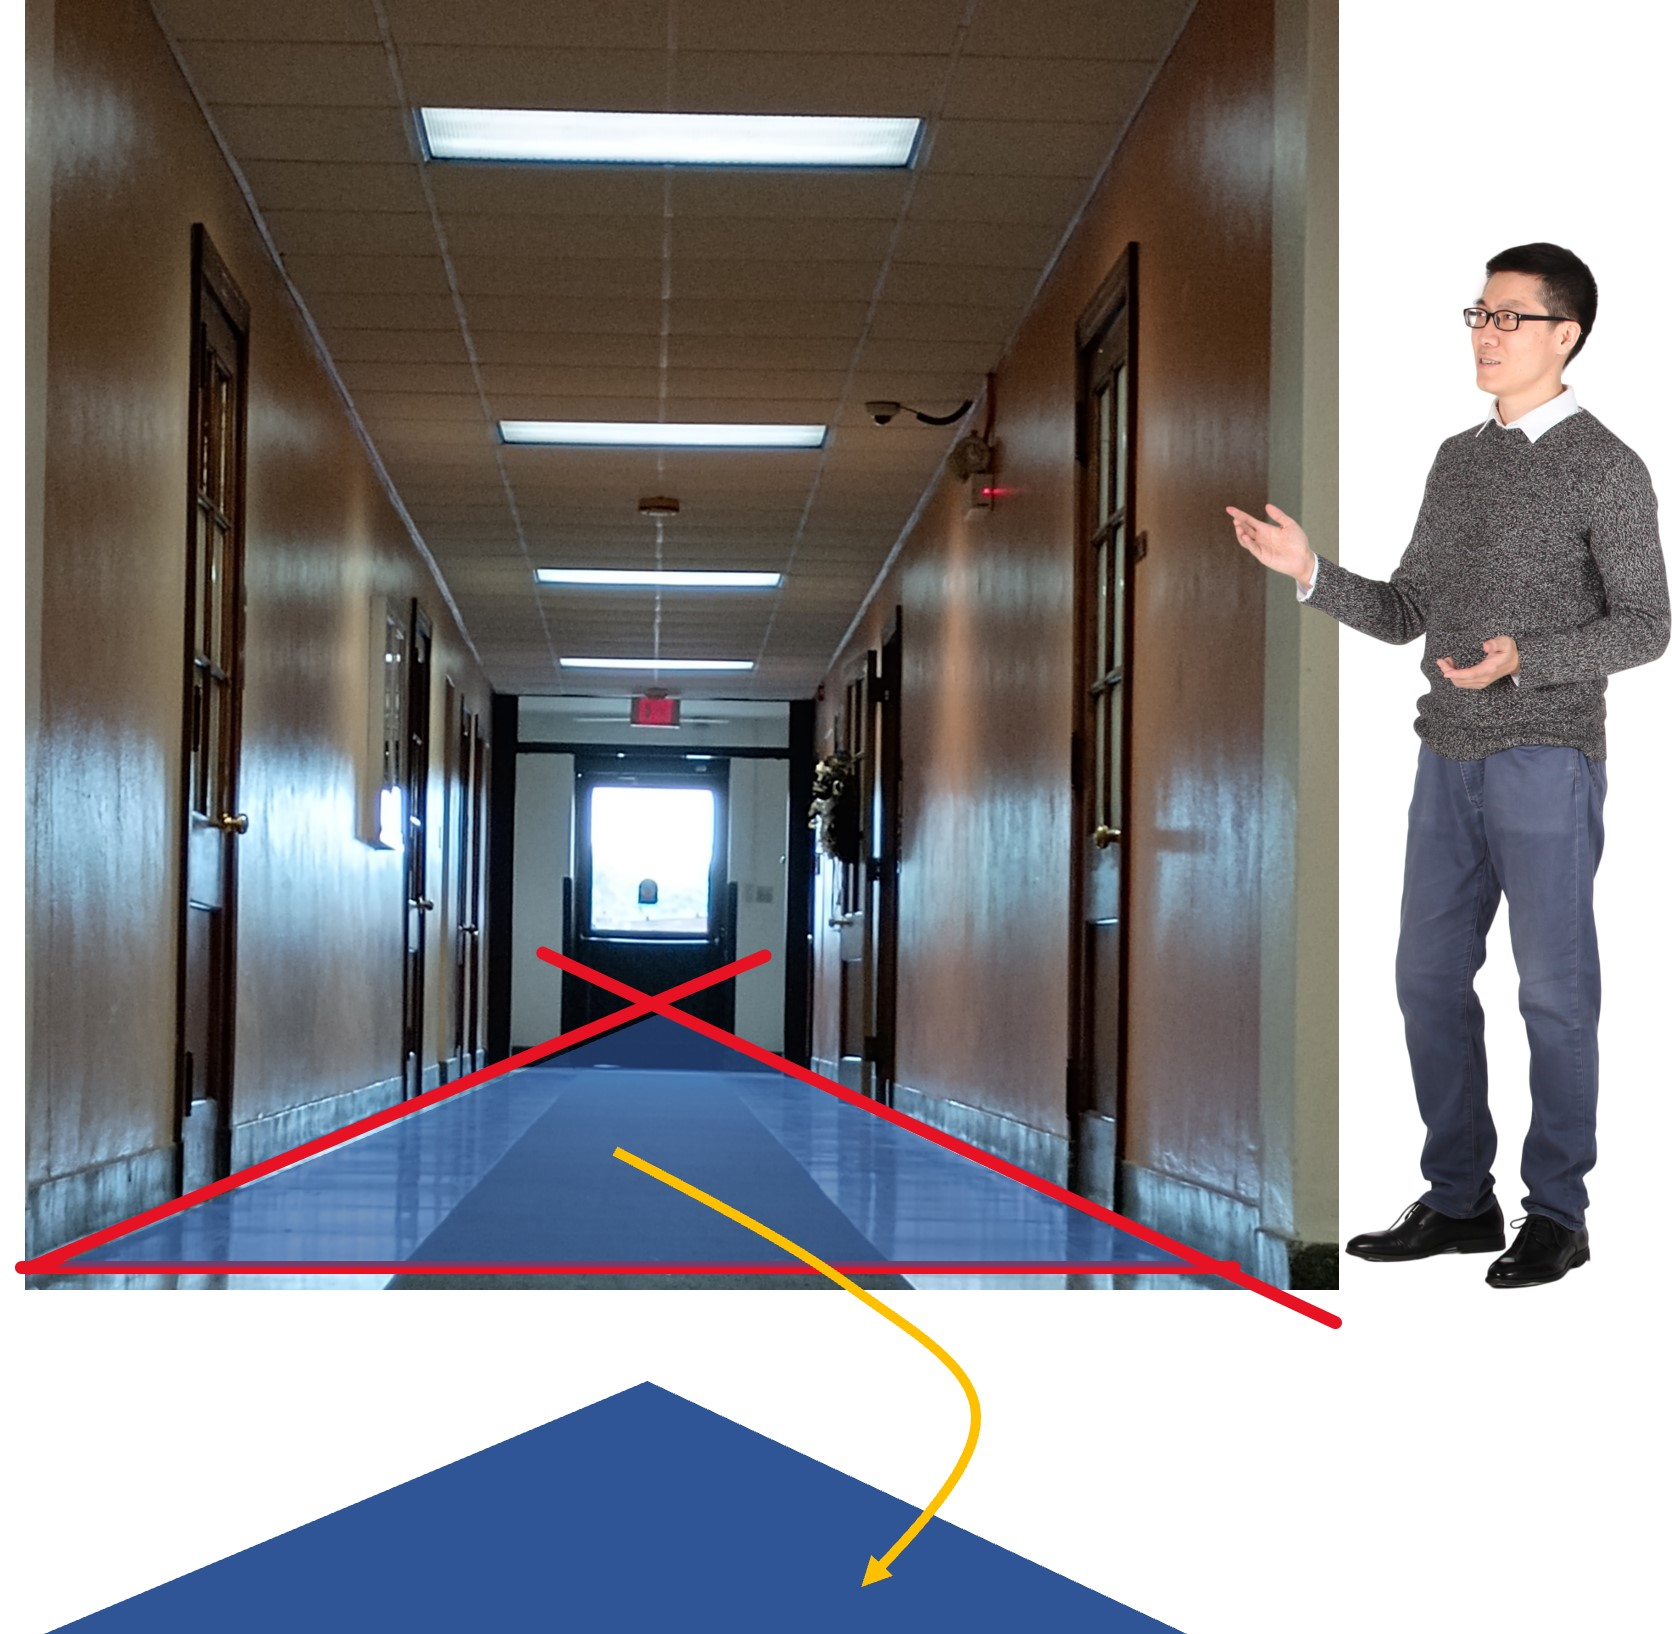
\includegraphics[width=4in]{lifeSize.jpg}
\end{image}

The interactive model below shows railroad tracks and the Eye (camera) looking at the tracks. The vertical plane is a picture plane.  The triangle in the picture plane is the image of the rails the Eye sees.  Note the location of the vanishing point. Observe how the sides of the triangle are formed by points of intersection of lines of sight with the picture plane.  You can rotate the model for a better view.  Use the slider to adjust the height of the Eye and note how the image in the picture plane changes.  

RIGHT-CLICK and DRAG to rotate the model for a better view.
\begin{center}
\geogebra{nakhdsae}{800}{600}
\end{center}

\textbf{Group Discussion Prompt:}
\emph{Explain why the height of the eye is the height of the triangle.}
\end{exploration}

\end{document}